%{
%Formattting
\documentclass[12pt,a4paper]{article}
\usepackage[T1]{fontenc}
\usepackage[utf8]{inputenc}
\usepackage[left=0.75in, right=0.75in, bottom=1.1in]{geometry}
\usepackage[skip=7pt plus1pt, indent=0pt]{parskip}

\usepackage{fancyheadings}
\usepackage{setspace}
\usepackage{enumitem}
\usepackage{longtable}
\usepackage{array} % include this in your preamble

\usepackage{multicol}
\setlength\columnseprule{0.4pt}
%\setlength{\parindent}{0in}
\usepackage{listings}

\lstset
{ %Formatting for code in appendix
	basicstyle=\footnotesize,
	numbers=left,
	stepnumber=1,
	showstringspaces=false,
	tabsize=1,
	breaklines=true,
	breakatwhitespace=false
}

\usepackage{xargs} 
\usepackage[pdftex,dvipsnames]{xcolor}

%Mathematics
\usepackage{amsmath}
\usepackage{amsthm}
\usepackage{amssymb}
\usepackage{polynom}
\usepackage{mathtools}
\usepackage{float}
\usepackage{aliascnt}

\newaliascnt{eqfloat}{equation}
\newfloat{eqfloat}{h}{eqflts}
\floatname{eqfloat}{Equation}
\newcommand*{\ORGeqfloat}{}
\let\ORGeqfloat\eqfloat
\def\eqfloat{%
	\let\ORIGINALcaption\caption
	\def\caption{%
		\addtocounter{equation}{-1}%
		\ORIGINALcaption
	}%
	\ORGeqfloat
}
\usepackage{upgreek}

\usepackage{pict2e}

%Professor Latex Commands:
\newcommand{\tr}{\mathrm{tr}}
\newcommand{\ra}{\rightarrow}
\newcommand{\lan}{\langle}
\newcommand{\ran}{\rangle}
\newcommand{\norm}[1]{\left\lVert#1\right\rVert}
\newcommand{\inn}[1]{\lan#1\ran}
\newcommand{\ol}{\overline}
\newcommand{\F}{\mathbf{F}}
\newcommand{\M}{\mathcal{M}}
\newcommand{\res}{\text{Res}}
\newcommand{\ds}{\displaystyle}
\newcommand{\range}{\text{range}}

\makeatletter
\newcommand{\crossout}[1]{%
	\begingroup
	\settowidth{\dimen@}{#1}%
	\setlength{\unitlength}{0.05\dimen@}%
	\settoheight{\dimen@}{#1}%
	\count@=\dimen@
	\divide\count@ by \unitlength
	\begin{picture}(0,0)
		\put(0,0){\line(20,\count@){20}}
		\put(0,\count@){\line(20,-\count@){20}}
	\end{picture}%
	#1%
	\endgroup
}
\usepackage{tikz}
\newcommand\halmos{\rule{.36em}{2ex}}
\newcommand{\powerset}[1]{\mathcal{P}(#1)}
\def\contradict{\tikz[baseline, x=0.22em, y=0.22em, line width=0.032em]\draw (0,2.83)--(2.83,0) (0.71,3.54)--(3.54,0.71) (0,0.71)--(2.83,3.54) (0.71,0)--(3.54,2.83);}

%Citations
%\usepackage{cite}
%\usepackage[backend=bibtex,style=verbose-trad2]{biblatex} %works really really well, but no MLA format
%\usepackage[backend=biber,style=mla]{biblatex} %Doesn't print all sources for some reason
%\addbibresource{references.bib}
%\bibliography{references.bib} 
\nocite{*}

%Symbols and Other
\usepackage{upgreek}
\usepackage{graphicx}
\usepackage{animate}
\usepackage{caption}
\newcommand{\source}[1]{\caption*{Source: {#1}} }
\usepackage{hyperref}
\hypersetup{
	colorlinks,
	allcolors=black
	%citecolor=black,
	%filecolor=black,
	%linkcolor=black,
	%urlcolor=black
}
%onehalfspacing
\linespread{1}
%\doublespacing

\pagestyle{fancy}
\headheight 32pt

\usepackage{pdfpages}
%}

% Drafting 
%{
\usepackage[colorinlistoftodos,prependcaption, textsize=tiny]{todonotes}
\usepackage{lipsum}
\newcommandx{\unsure}[2][1=]{\todo[linecolor=red,backgroundcolor=red!25,bordercolor=red,#1]{#2}}
\newcommandx{\change}[2][1=]{\todo[linecolor=blue,backgroundcolor=blue!25,bordercolor=blue,#1]{#2}}
\newcommandx{\toadd}[2][1=]{\todo[linecolor=OliveGreen,backgroundcolor=OliveGreen!25,bordercolor=OliveGreen,#1]{#2}}
\newcommandx{\info}[2][1=]{\todo[linecolor=yellow,backgroundcolor=yellow!25,bordercolor=yellow,#1]{#2}}
\newcommandx{\improve}[2][1=]{\todo[linecolor=Plum,backgroundcolor=Plum!25,bordercolor=Plum,#1]{#2}}
\newcommandx{\hiddentodo}[2][1=]{\todo[disable,#1]{#2}}
%}
% ========================================= %
% Change for each document [!!!]
\newcommand\team{University of Toronto Aerospace Team}	%Class Code [!!!]
\newcommand\doctitle{Subsystem Design Specification} %LAB REPORT TITLE [!!!]
\newcommand\subteam{Onboard Computer}  

% https://q.utoronto.ca/courses/328612/files/27127427?module_item_id=4885895
\pagenumbering{gobble}
\begin{document}
    \title{\doctitle}
	\author{\team \\ \subteam}
	%\date{\textbf{TA:} \taname \\ \textbf{Location:} \location \\ \textbf{Date:} DATE} %Put in date of submission [!!!]

	\maketitle
	
	\tableofcontents
    \thispagestyle{empty}
	
	\newpage
    \clearpage
    \pagenumbering{arabic}
    %So the heading doesn't show up on table of contents page
	%\lhead{\yourname\ \vspace{0.1cm} \\ \course}
	\lhead{\subteam}
    \chead{\textbf{\doctitle}}
    \rhead{July, 2025}

    \section{Subteam Overview}
    \subsection{Technical Responsibilities}
    The electrical team has two main deliverables for the spacecraft:
    \begin{enumerate}
        \item The OnBoard Computer (OBC)
        \item The Payload Controller (PAY)
    \end{enumerate}
    Each deliverable is an STM32-based PCB that is designed, validated, and tested in-house. 
    
    As the board is being designed in house, the team is also responsible for:
    \begin{itemize}
        \item Ensuring boards can be manufactured for flight when the time comes
        \item Creating and maintaining datasheets for each board
        \item Maintaining the Interface Control Document
    \end{itemize}

    \subsection{Other Responsibilities}
    \begin{itemize}
        \item Training up members of the subteam to work on OBC and PAY via onboarding projects.
        \item Maintaining the Altium library-- ensuring that all components can withstand the space environment. 
        \item Maintaining the lab space (MY618) for electrical testing and PCB bring-up. 
        \item Placing PCB fabrication and component orders
    \end{itemize}
    
    
    \section{Applicable Documents and Standards}\label{sec:methods}
    \subsection{Technical Documents}
    \begin{itemize}
        \item OBC Datasheet
        \item PAY Datasheet
        \item Master Connection Sheet
    \end{itemize}
    \subsection{Standards Documents}
   
    \section{Subsystem Requirements}\label{sec:requirements}

    \subsection{Electrical System Requirements}
    From the FINCH-Spacecraft-ElectricalSystem, requirements for the existence of OBC and PAY are derived. Seen in Table \ref{tab:elec_sys_req} are also other higher-lever requirements of the system including the common bus to connect OBC, PAY, and the board for the Electrical Power System (EPS).
    \begin{table}[H]
        \centering
        \begin{tabular}{|>{\centering\arraybackslash}m{3cm} 
                    |>{\raggedright\arraybackslash}m{7cm} 
                    |>{\centering\arraybackslash}m{3cm} 
                    |>{\centering\arraybackslash}m{2.5cm}|}\hline
            \textbf{Req. ID} & \centering \textbf{Description} & \textbf{Parent Req.} & \textbf{Verification Method}\\\hline
             FINCH-Spacecraft-ElectricalSystem&  The electrical system shall provide the necessary electrical functionality for the mission to function. &  FINCH-Mission-Objective& Demonstration\\\hline
 FINCH-OBC-ControlAndOps& The OBC shall control the modes of operation of the satellite. & FINCH-Spacecraft-ElectricalSystem&Demonstration\\\hline
 FINCH-Payload Controller-PayloadOps& The Payload Controller shall support necessary operations for executing the mission of the payload& FINCH-Spacecraft-ElectricalSystem&Demonstration\\\hline
             FINCH-Spacecraft-CommonBus&  The spacecraft shall utilize a common bus which includes the lines for power and communication between OBC, EPS, and PAY. &  FINCH-Spacecraft-ElectricalSystem& Test\\\hline
             FINCH-Spacecraft-CANBus&  The spacecraft shall use CAN Bus for communication between nodes on the electrical system.&  FINCH-Spacecraft-CommonBus& Test\\\hline
             FINCH-Spacecraft-Electrical Grounding&  The grounding system for the spacecraft shall include a separate chassis and signal ground.&  FINCH-Spacecraft-ElectricalSystem& Analysis\\\hline
             FINCH-Spacecraft-Electrical Soldering Standard&  Electrical components shall be soldered in accordance to IPC Type 3 or equivalent&  FINCH-Spacecraft-ElectricalSystem& Inspection\\\hline
        \end{tabular}
        \caption{Electrical System Requirements}\label{tab:elec_sys_req}
    \end{table}

    \subsection{OBC Requirements}
    \begin{figure}[H]
        \centering
        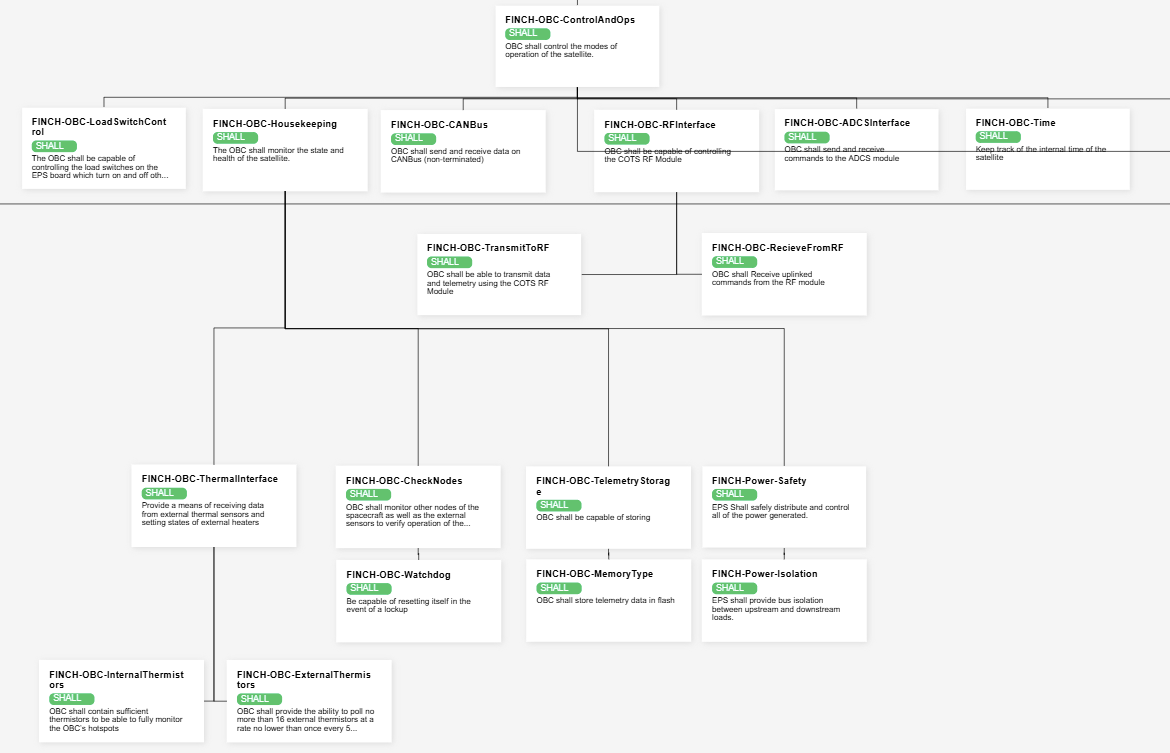
\includegraphics[width=0.98\linewidth]{../figures/OBC_req_tree.png}
        \caption{Requirement tree view of the requirements for the OnBoard Computer}
        \label{fig:OBC_req_tree}
    \end{figure}
    
    \begin{table}[H]
        \centering
        \begin{tabular}{|>{\centering\arraybackslash}m{3cm} 
                    |>{\raggedright\arraybackslash}m{7cm} 
                    |>{\centering\arraybackslash}m{3cm} 
                    |>{\centering\arraybackslash}m{2.5cm}|}\hline
            \textbf{Req. ID} & \centering \textbf{Description} & \textbf{Parent Req.} & \textbf{Verification Method}\\\hline
             FINCH-OBC-LoadSwitch Control&      The OBC shall be capable of controlling the load switches on the EPS board which turn on and off other nodes on the satellite (&  FINCH-OBC-ControlAndOps& Demonstration\\\hline
             FINCH-OBC-CANBus&  The OBC shall send and receive data on CANBus (non-terminated)&  FINCH-OBC-ControlAndOps, FINCH-Spacecraft-CANBus& Test\\\hline
             FINCH-OBC-Time&  The OBC shall track of the internal time of the satellite&  FINCH-OBC-ControlAndOps& Test\\\hline
             FINCH-OBC-Housekeeping&  The OBC shall monitor the state and health of the satellite.&  FINCH-OBC-ControlAndOps& Test\\\hline
             FINCH-OBC-CheckNodes&  OBC shall monitor other nodes of the spacecraft as well as the external sensors to verify operation of the spacecraft is going without fault. &  FINCH-OBC-Housekeeping& Test, Analysis\\\hline
             FINCH-OBC-Watchdog&  The OBC shall be capable of resetting itself in the event of a lockup&  FINCH-OBC-CheckNodes& Test\\ \hline
 FINCH-OBC-TelemetryStorage& The OBC shall be capable of storing telemetry and housekeeping data.& FINCH-OBC-Housekeeping&Test\\\hline
 FINCH-OBC-MemoryType& The OBC shall store telemetry data flash memory.& FINCH-OBC-TelemetryStorage&Test\\\hline
 FINCH-OBC-ThermalInterface& Provide a means of receiving data from external thermal sensors and setting states of external heaters& FINCH-OBC-Housekeeping&Test\\\hline
 FINCH-OBC-Internal Thermistors& The OBC shall contain sufficient thermistors to be able to fully monitor the OBC’s hotspots.& FINCH-OBC-ThermalInterface&Test\\\hline
 FINCH-OBC-External Thermistors& The OBC shall provide the ability to poll no more than 16 external thermistors at a rate no lower than once every 5 seconds.& FINCH-OBC-ThermalInterface&Test\\\hline
        \end{tabular}
        \caption{OBC Requirements}
        \label{tab:placeholder}
    \end{table}
    \subsection{PAY Requirements}
Figure \ref{fig:PAY_req_tree} and Table \ref{tab:pay_reqs}
summarize the requirements for the Payload Controller system. 

Notable is the compression requirement which has only become a "should" recently after PAY was designed. The reason why the requirement suddenly became a "should" comes from a spec from optics saying that the whole sensor will not be used. Initial requirement for compression assumed the whole sensor would be used. 
    \begin{figure}[H]
        \centering
        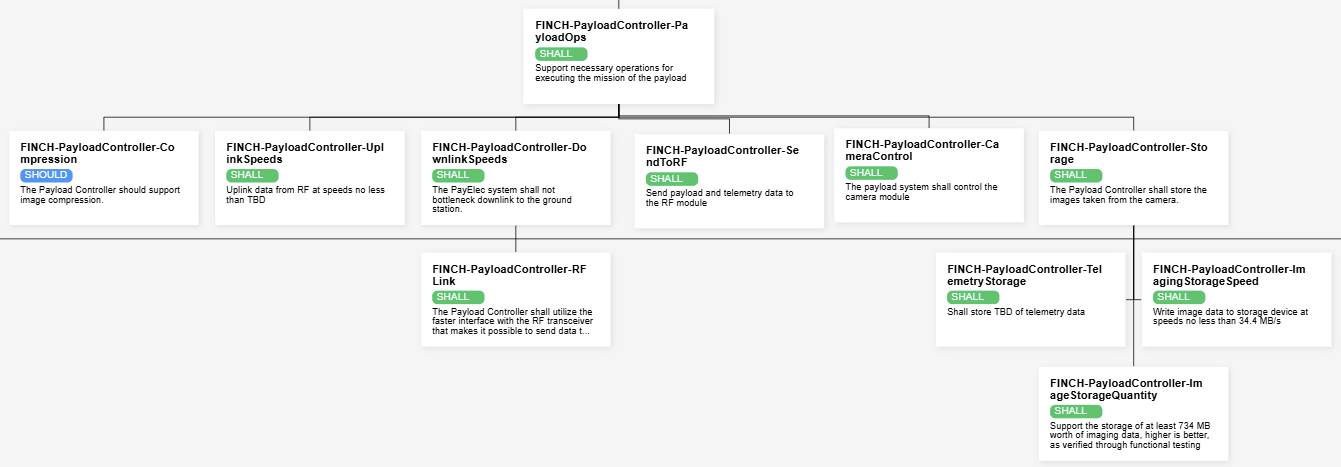
\includegraphics[width=1\linewidth]{../figures/PAY_req_tree.png}
        \caption{PAY Requirement Tree}
        \label{fig:PAY_req_tree}
    \end{figure}

    \begin{table}[H]
        \centering
        \begin{tabular}{|>{\centering\arraybackslash}m{3cm} 
                    |>{\raggedright\arraybackslash}m{7cm} 
                    |>{\centering\arraybackslash}m{3cm} 
                    |>{\centering\arraybackslash}m{2.5cm}|}\hline
            \textbf{Req. ID} & \centering \textbf{Description} & \textbf{Parent Req.} & \textbf{Verification Method}\\\hline
 FINCH-PayloadController-CameraControl& The Payload Controller shall control the camera module& FINCH-PayloadController-PayloadOps&Test, Analysis\\\hline
 FINCH-PayloadController-Storage& The Payload Controller shall store the images taken from the camera.& FINCH-PayloadController-Storage&Test\\\hline
 FINCH-PayloadController-ImagingStorageSpeed& The Payload Controller shall write image data to storage device at speeds no less than 34.4 MB/s& FINCH-PayloadController-Storage&Test\\\hline
 FINCH-PayloadController-ImageStorageQuantity& The Payload Controller shall support the storage of at least 734 MB worth of imaging data, higher is better, as verified through functional testing& FINCH-PayloadController-Storage&Test\\\hline
 FINCH-PayloadController-TelemetryStorage& The Payload Controller shall be capable of storing telemetry data.& FINCH-PayloadController-Storage&Test\\\hline
 FINCH-PayloadController-DownlinkSpeeds& The Payload Controller system shall not bottleneck downlink to the ground station. & FINCH-PayloadController-PayloadOps&Test\\\hline
 FINCH-PayloadController-RFLink& The Payload Controller shall utilize the faster interface with the RF transceiver that makes it possible to send data to the transceiver such that it does not bottleneck communication.& FINCH-PayloadController-DownlinkSpeeds&Test\\\hline
 FINCH-PayloadController-UplinkSpeeds& The Payload Controller system shall be capable of receiving data from the RF module directly. & FINCH-PayloadController-PayloadOps&Test\\\hline
 FINCH-PayloadController-SendToRF& The Payload Controller shall be capable of directly sending payload and telemetry data to the RF module.& FINCH-PayloadController-PayloadOps&Test\\\hline
 FINCH-PayloadController-Compression& The Payload Controller should support image compression.& FINCH-PayloadController-PayloadOps&Test\\\hline
        \end{tabular}
        \caption{Electrical System Requirements}\label{tab:pay_reqs}
    \end{table}

   
    
    \section{Verification and Validation Plan}\label{sec:verifcation_validation}
    Electrical requirements will be verified via tests and demonstrations. The verification and validation plan will follow the following timeline:
    


    \section{High Level System Architecture}

    \section{Detailed System Architecture}

    \section{Possible Risks}

    \section{Development Schedule and Status}

    \section{Open Issues and Future Work}
    
            
    \newpage
    \pagenumbering{roman}


    %\section{Uncertainty Calculations}




\end{document}

\begin{figure}[h]
            \centering
             \begin{minipage}{0.49\linewidth}
                \centering
                \includegraphics[width=1\textwidth]{left figure}
                \caption{\centering left caption}
                \label{fig:left_fig}
            \end{minipage}
            \begin{minipage}{0.49\linewidth}
                \centering
                \includegraphics[width=1\textwidth]{right figure}
                \caption{\centering right caption}
                \label{fig:right_fig}
            \end{minipage}
      \end{figure}

          % \begin{equation}
    %     \begin{split}
    %         Z_{in} &= \left( \frac{1}{r_b} + \frac{1}{Z_{base}} \right)^{-1} \\
    %         &= \left( \frac{1}{r_b} + \frac{i_b}{i_e (r'_e + R_{sw}))} \right)^{-1} 
    %     \end{split}
    % \end{equation}

    % $i_e = i_c + i_b = i_b(\beta + 1)\approx \beta i_b = i_c$ for $\beta \gg 1$. This approximation often holds as $\beta$ is usually large. Making this approximation,

    % \begin{equation}
    %     \begin{split}
    %         Z_{in} &= \left( \frac{1}{r_b} + \frac{1}{\beta (r'_e + R_{sw})} \right)^{-1} \\
    %          &= \frac{\beta r_b(r'_e + R_{sw})}{\beta (r'_e + R_{sw}) + r_b}
    %     \end{split}
    % \end{equation}
    
    % \begin{equation}
    %     A_V = \frac{v_{out}}{v_{in}} = \frac{-r_c i_c}{i_e }
    % \end{equation}

    % The gain of 

    % From Equation \eqref{eqn:r'_e}, $i_c$ must be determined to solve for $r'_e$. From Equation \eqref{eqn:transistor_eqn}, $i_c$ can be found knowing $i_b$. By Kirchoff's voltage law on the loop containing $r_b$, $r'_e$, and $R_{sw}$ on the AC equivalent circuit, 
    % \begin{equation}
    %     r_b i_b = (r'_e + R_{sw})i_e 
    % \end{equation}
    % $i_e = i_c + i_b = i_b(\beta + 1)\approx \beta i_b = i_c$ for $\beta \gg 1$. This approximation often holds as $\beta$ is usually large. Making this approximation,
    % \begin{equation}
    %     \begin{split}
    %         i_c &= \frac{r_b i_b}{(r'_e + R_{sw})}\\
    %          %&= \frac{r_b}{\beta{(r'_e + R_{sw})}}
    %          \label{eqn:collector_current}
    %     \end{split}
    % \end{equation}
    % Using this in equation \eqref{eqn:r'_e},
    % \begin{equation}
    %     r'_e = \frac{R_{sw}}{\frac{r_b}{\beta \kappa_T} }
    % \end{equation}
